\documentclass[tikz,border=2pt]{standalone}
\usepackage{amsmath,amssymb}
\usepackage{tikz}
\usetikzlibrary{arrows.meta}

\begin{document}
% Objective lines z = 3 x_s + 2 x_t = const: parallel lines of slope -3/2 that move away
% from the origin as z grows; the gradient (3, 2) is perpendicular to them.
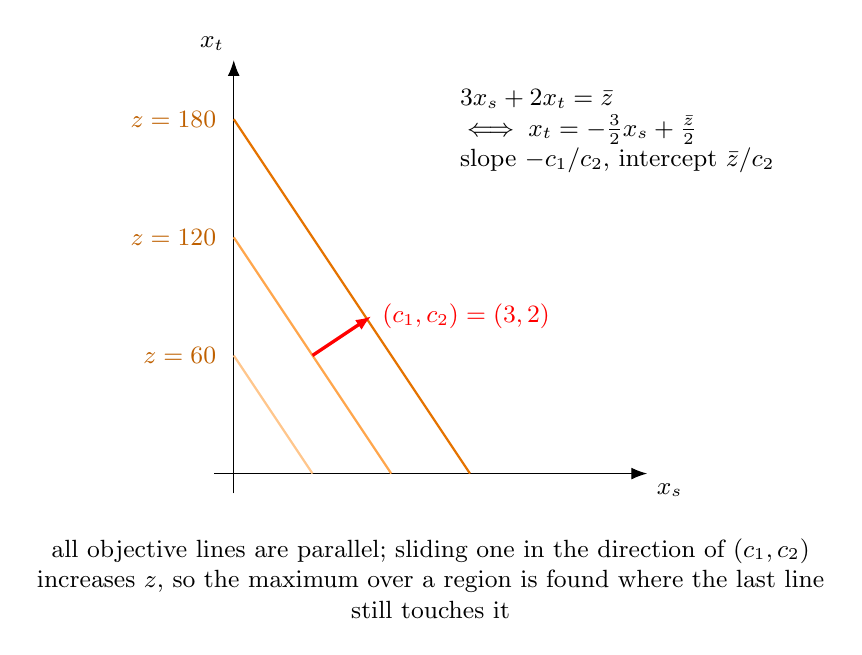
\begin{tikzpicture}[x=0.05cm, y=0.05cm, every node/.style={font=\small}, >={Latex[length=2mm]}]
	\draw[->] (-5,0) -- (105,0) node[below right] {$x_s$};
	\draw[->] (0,-5) -- (0,105) node[above left] {$x_t$};
	\foreach \z/\c in {60/orange!45, 120/orange!70, 180/orange!90!black} {
		\pgfmathsetmacro{\xa}{\z/3}
		\pgfmathsetmacro{\yb}{\z/2}
		\draw[\c, thick] (\xa,0) -- (0,\yb);
		\node[orange!75!black, anchor=east] at (-2,\yb) {$z=\z$};
	}
	\draw[->, red, very thick] (20,30) -- (35,40) node[right, font=\small] {$(c_1,c_2)=(3,2)$};
	\node[anchor=north west, font=\small, align=left] at (55,100) {$3x_s+2x_t=\bar z$\\ $\iff x_t=-\tfrac32x_s+\tfrac{\bar z}{2}$\\ slope $-c_1/c_2$, intercept $\bar z/c_2$};
	\node[anchor=north, align=flush center, text width=10cm] at (50,-14) {all objective lines are parallel; sliding one in the direction of $(c_1,c_2)$ increases $z$, so the maximum over a region is found where the last line still touches it};
\end{tikzpicture}
\end{document}
